\documentclass[12pt,space]{ctexart} %ans
\usepackage{GKExam}
\begin{document}\zihao{5}
\juemi% 输出绝密
\biaoti{2020年普通高等学校招生全国统一考试}
\fubiaoti{文科数学}
\renewcommand{\filename}{文科数学试题}
{\heiti 注意事项}:
\begin{enumerate}[itemsep=-0.3em,topsep=0pt]
\item 答卷前,考生务必将自己的姓名、准考证号填写在答题卡上. 
\item 回答选择题时,选出每小题答案后,用铅笔把答题卡对应题目的答案标号涂黑. 如需改动,用橡皮擦干净后,再选涂其它答案标号. 回答非选择题时,将答案写在答题卡上. 写在本试卷上无效. 
\item 考试结束后,将本试卷和答题卡一并交回. 请认真核对监考员在答题卡上所粘贴的条形码上的姓名、准考证号与您本人是否相符. 
\end{enumerate}

\section{选择题:本大题共12小题,每小题5分,共60分. 在每小题给出的四个选项中,只有一项是符合题目要求的. }
\begin{enumerate}[itemsep=0.2em,topsep=0pt]

  \item 集合$M=\{2,4,6,8,10\}$,$N=\{x \mid-1<x<6\}$,则$M\cap N$= 
  \begin{tasks}(4)
    \task $\{2,4\}$ \task $\{2,4,6\}$ \task $\{2,4,6,8\}$ \task $\{2,4,6,8,10\}$ 
  \end{tasks}

  \item 设$(1+2i)a+b=2i$,其中$a$,$b$为实数,则
  \begin{tasks}(4)
    \task $a=1$,$b=-1$ \task $a=1$,$b=1$ \task $a=-1$,$b=1$ \task $a=-1$,$b=-1$  
  \end{tasks}

  \item 分别统计了甲、乙两位同学16周的各周课外体育运动时长(单位:h),得如下茎叶图:\\[-1.5em]
  \begin{figure}[htbp]
    \centering
    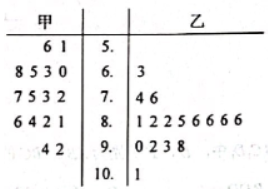
\includegraphics{Image/ii-w-3.png}
  \end{figure}\\[-1.5em]
  则下列结论中错误的是
  \begin{tasks}(1)
    \task 甲同学周课外体育运动时长的样本中位数为7.4
    \task 乙同学周课外体育运动时长的样本平均数大于8
    \task 甲同学周课外体育运动时长大于8的概率的估计值大于0.4
    \task 乙同学周课外体育运动时长大于8的概率的估计值大于0.6
  \end{tasks}

  \item 若$x$,$y$满足约束条件$\left\{\begin{array}{l}x+y\geqslant 2,\\x+2y\leqslant 4,\\y\geqslant 0,\end{array}\right.$则$z=2x-y$的最大值是
  \begin{tasks}(4)
    \task -2 \task 4 \task 8 \task 12
  \end{tasks}

  \item 设$F$为抛物线$C:y^{2}=4x$的焦点,点$A$在$C$上,点$B(3,0)$,若$|AF|=|BF|$,则$|AB|=$
  \begin{tasks}(4)
    \task 2 \task $2\sqrt{2}$ \task 3 \task $3\sqrt{2}$
  \end{tasks}

  \begin{minipage}[h][42ex][t]{.40\textwidth}
    \item 执行右边的程序框图,输出的$n=$
    \begin{tasks}(1)
      \task 3
      \task 4
      \task 5
      \task 6
    \end{tasks}
  \end{minipage}
  \begin{minipage}[h][42ex][t]{.55\textwidth}
    \flushright
    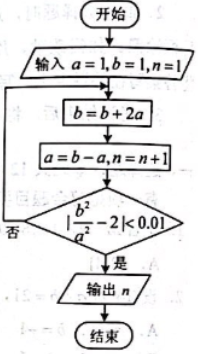
\includegraphics[width=.4\textwidth]{Image/ii-w-7.png}
  \end{minipage}


  \begin{minipage}[h][24ex][t]{.70\textwidth}
    \item 右图是下列四个函数中的某个函数在区间$[-3,3]$的大致图像,则该函数是
    \begin{tasks}(1)
      \task  $y=\displaystyle{\frac{-x^{3}+3x}{x^{2}+1}}$
      \task  $y=\displaystyle{\frac{x^{3}-x}{x^{2}+1}}$
      \task  $y=\displaystyle{\frac{2x\cos x}{x^{2}+1}}$
      \task  $y=\displaystyle{\frac{2\sin x}{x^{2}+1}}$
    \end{tasks}
  \end{minipage}
  \begin{minipage}[h][24ex][t]{.30\textwidth}
    \flushright
    \vspace{3em}
    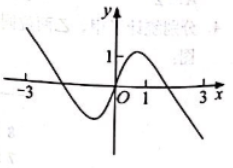
\includegraphics[width=0.7\textwidth]{Image/ii-w-8.png}
    \hspace{2em}
  \end{minipage}

  \item 在正方体$ABCD-A_1B_1C_1D_1$中,$E$,$F$分别为$AB$,$BC$的中点,则
  \begin{tasks}(2)
    \task 平面$B_1EF\bot $平面$BDD_1$
    \task 平面$B_1EF\bot $平面$A_1BD$
    \task 平面$B_1EF\varparallel$平面$A_1AC$
    \task 平面$B_1EF\varparallel$平面$A_1C_1D$
  \end{tasks}

  \item 已知等比数列$\{a_n\}$的前3相和为168,$a_2-a_5=42$,则$a_6=$
  \begin{tasks}(4)
    \task 14 \task 12 \task 6 \task 3
  \end{tasks}

  \item 函数$f(x)=\cos x+(x+1)\sin x+1$在区间$[0, 2\pi]$的最小值和最大值分别为
  \begin{tasks}(4)
    \task $\displaystyle{-\frac{\pi}{2}}$,$\displaystyle{\frac{\pi}{2}}$
    \task $\displaystyle{-\frac{3\pi}{2}}$,$\displaystyle{\frac{\pi}{2}}$
    \task $\displaystyle{-\frac{\pi}{2}}$,$\displaystyle{\frac{\pi}{2}+2}$
    \task $\displaystyle{-\frac{3\pi}{2}}$,$\displaystyle{\frac{\pi}{2}+2}$
  \end{tasks}

  \item 已知球$O$的半径为1,四棱锥的顶点为$O$,底面上的四个顶点均在球$O$的球面上,则当这个四棱锥的体积最大时,其高为
  \begin{tasks}(4)
   \task $\displaystyle{\frac 13}$
   \task $\displaystyle{\frac 12}$
   \task $\displaystyle{\frac {\sqrt{3}}{3}}$
   \task $\displaystyle{\frac {\sqrt{2}}{2}}$
  \end{tasks}

\end{enumerate}

\section{填空题:本大题共4小题,每小题5分,共20分.}
\begin{enumerate}[itemsep=0.2em,topsep=0pt, resume]

  \item 记$S_n$为等差数列$\{a_n\}$的前$n$项和. 若$2S_3=3S_2+6$,则公差$d=$\blank{2}.

\end{enumerate}

\clearpage
\end{document}